
% --- LaTeX Homework Template - S. Venkatraman ---

% --- Set document class and font size ---

\documentclass[letterpaper, 11pt]{article}

% --- Package imports ---

\usepackage{
  amsmath, amsthm, amssymb, mathtools, dsfont,	  % Math typesetting
  graphicx, wrapfig, subfig, float,                  % Figures and graphics formatting
  listings, color, inconsolata, pythonhighlight,     % Code formatting
  fancyhdr, sectsty, hyperref, enumerate, enumitem } % Headers/footers, section fonts, links, lists

% --- Page layout settings ---

% Set page margins
\usepackage[left=1.35in, right=1.35in, bottom=1in, top=1.1in, headsep=0.2in]{geometry}

% Anchor footnotes to the bottom of the page
\usepackage[bottom]{footmisc}

% Set line spacing
\renewcommand{\baselinestretch}{1.2}

% Set spacing between paragraphs
\setlength{\parskip}{1.5mm}

% Allow multi-line equations to break onto the next page
\allowdisplaybreaks

% Enumerated lists: make numbers flush left, with parentheses around them
\setlist[enumerate]{wide=0pt, leftmargin=21pt, labelwidth=0pt, align=left}
\setenumerate[1]{label={(\arabic*)}}

% --- Page formatting settings ---

% Set link colors for labeled items (blue) and citations (red)
\hypersetup{colorlinks=true, linkcolor=blue, citecolor=red}

% Make reference section title font smaller
\renewcommand{\refname}{\large\bf{References}}

% --- Settings for printing computer code ---

% Define colors for green text (comments), grey text (line numbers),
% and green frame around code
\definecolor{greenText}{rgb}{0.5, 0.7, 0.5}
\definecolor{greyText}{rgb}{0.5, 0.5, 0.5}
\definecolor{codeFrame}{rgb}{0.5, 0.7, 0.5}

% Define code settings
\lstdefinestyle{code} {
  frame=single, rulecolor=\color{codeFrame},            % Include a green frame around the code
  numbers=left,                                         % Include line numbers
  numbersep=8pt,                                        % Add space between line numbers and frame
  numberstyle=\tiny\color{greyText},                    % Line number font size (tiny) and color (grey)
  commentstyle=\color{greenText},                       % Put comments in green text
  basicstyle=\linespread{1.1}\ttfamily\footnotesize,    % Set code line spacing
  keywordstyle=\ttfamily\footnotesize,                  % No special formatting for keywords
  showstringspaces=false,                               % No marks for spaces
  xleftmargin=1.95em,                                   % Align code frame with main text
  framexleftmargin=1.6em,                               % Extend frame left margin to include line numbers
  breaklines=true,                                      % Wrap long lines of code
  postbreak=\mbox{\textcolor{greenText}{$\hookrightarrow$}\space} % Mark wrapped lines with an arrow
}

% Set all code listings to be styled with the above settings
\lstset{style=code}

% --- Math/Statistics commands ---

% Add a reference number to a single line of a multi-line equation
% Usage: "\numberthis\label{labelNameHere}" in an align or gather environment
\newcommand\numberthis{\addtocounter{equation}{1}\tag{\theequation}}

% Shortcut for bold text in math mode, e.g. $\b{X}$
\let\b\mathbf

% Shortcut for bold Greek letters, e.g. $\bg{\beta}$
\let\bg\boldsymbol

% Shortcut for calligraphic script, e.g. %\mc{M}$
\let\mc\mathcal

% \mathscr{(letter here)} is sometimes used to denote vector spaces
\usepackage[mathscr]{euscript}

% Convergence: right arrow with optional text on top
% E.g. $\converge[w]$ for weak convergence
\newcommand{\converge}[1][]{\xrightarrow{#1}}

% Normal distribution: arguments are the mean and variance
% E.g. $\normal{\mu}{\sigma}$
\newcommand{\normal}[2]{\mathcal{N}\left(#1,#2\right)}

% Uniform distribution: arguments are the left and right endpoints
% E.g. $\unif{0}{1}$
\newcommand{\unif}[2]{\text{Uniform}(#1,#2)}

% Independent and identically distributed random variables
% E.g. $ X_1,...,X_n \iid \normal{0}{1}$
\newcommand{\iid}{\stackrel{\smash{\text{iid}}}{\sim}}

% Equality: equals sign with optional text on top
% E.g. $X \equals[d] Y$ for equality in distribution
\newcommand{\equals}[1][]{\stackrel{\smash{#1}}{=}}

% Math mode symbols for common sets and spaces. Example usage: $\R$
\newcommand{\R}{\mathbb{R}}   % Real numbers
\newcommand{\C}{\mathbb{C}}   % Complex numbers
\newcommand{\Q}{\mathbb{Q}}   % Rational numbers
\newcommand{\Z}{\mathbb{Z}}   % Integers
\newcommand{\N}{\mathbb{N}}   % Natural numbers
\newcommand{\F}{\mathcal{F}}  % Calligraphic F for a sigma algebra
\newcommand{\El}{\mathcal{L}} % Calligraphic L, e.g. for L^p spaces

% Math mode symbols for probability
\newcommand{\pr}{\mathbb{P}}    % Probability measure
\newcommand{\E}{\mathbb{E}}     % Expectation, e.g. $\E(X)$
\newcommand{\var}{\text{Var}}   % Variance, e.g. $\var(X)$
\newcommand{\cov}{\text{Cov}}   % Covariance, e.g. $\cov(X,Y)$
\newcommand{\corr}{\text{Corr}} % Correlation, e.g. $\corr(X,Y)$
\newcommand{\B}{\mathcal{B}}    % Borel sigma-algebra

% Other miscellaneous symbols
\newcommand{\tth}{\text{th}}	% Non-italicized 'th', e.g. $n^\tth$
\newcommand{\Oh}{\mathcal{O}}	% Big-O notation, e.g. $\O(n)$
\newcommand{\1}{\mathds{1}}	% Indicator function, e.g. $\1_A$

% Additional commands for math mode
\DeclareMathOperator*{\argmax}{argmax}    % Argmax, e.g. $\argmax_{x\in[0,1]} f(x)$
\DeclareMathOperator*{\argmin}{argmin}    % Argmin, e.g. $\argmin_{x\in[0,1]} f(x)$
\DeclareMathOperator*{\spann}{Span}       % Span, e.g. $\spann\{X_1,...,X_n\}$
\DeclareMathOperator*{\bias}{Bias}        % Bias, e.g. $\bias(\hat\theta)$
\DeclareMathOperator*{\ran}{ran}          % Range of an operator, e.g. $\ran(T) 
\DeclareMathOperator*{\dv}{d\!}           % Non-italicized 'with respect to', e.g. $\int f(x) \dv x$
\DeclareMathOperator*{\diag}{diag}        % Diagonal of a matrix, e.g. $\diag(M)$
\DeclareMathOperator*{\trace}{trace}      % Trace of a matrix, e.g. $\trace(M)$

% Numbered theorem, lemma, etc. settings - e.g., a definition, lemma, and theorem appearing in that 
% order in Section 2 will be numbered Definition 2.1, Lemma 2.2, Theorem 2.3. 
% Example usage: \begin{theorem}[Name of theorem] Theorem statement \end{theorem}
\theoremstyle{definition}
\newtheorem{theorem}{Theorem}[section]
\newtheorem{proposition}[theorem]{Proposition}
\newtheorem{lemma}[theorem]{Lemma}
\newtheorem{corollary}[theorem]{Corollary}
\newtheorem{definition}[theorem]{Definition}
\newtheorem{example}[theorem]{Example}
\newtheorem{remark}[theorem]{Remark}

% Un-numbered theorem, lemma, etc. settings
% Example usage: \begin{lemma*}[Name of lemma] Lemma statement \end{lemma*}
\newtheorem*{theorem*}{Theorem}
\newtheorem*{proposition*}{Proposition}
\newtheorem*{lemma*}{Lemma}
\newtheorem*{corollary*}{Corollary}
\newtheorem*{definition*}{Definition}
\newtheorem*{example*}{Example}
\newtheorem*{remark*}{Remark}
\newtheorem*{claim}{Claim}

% --- Left/right header text (to appear on every page) ---

% Include a line underneath the header, no footer line
\pagestyle{fancy}
\renewcommand{\footrulewidth}{0pt}
\renewcommand{\headrulewidth}{0.4pt}

% Left header text: course name/assignment number
\lhead{MATH-UA 228 (Fundamental Dynamics of Earth’s Atmosphere and Climate) -- Homework 2}

% Right header text: your name
\rhead{Yixia Yu (yy5091@nyu.edu)}

% --- Document starts here ---

\begin{document}
\begin{enumerate}[leftmargin=*, label=\arabic*.]

  \item NFL regulations stipulate that a football must be inflated to a pressure between 12.5 and 13.5 psi (pounds per square inch). An unnamed team might have "accidentally" inflated their football to 12.5 psi in a very warm locker room, $T = 25^\circ$C or $77^\circ$F. Determine the pressure inside the ball when playing at near freezing temperature ($T = 0^\circ$C), assuming that the volume of the ball remains the same and no air has leaked out. Note that psi is one of these old measuring units -- only used nowadays for pressure in tires and balls. You can solve this problem without converting to Pascal, or you can convert to Pa, do the calculations, and convert back to psi at the end.

  \item Here our goal is to compare the boiling point of water in Denver (air pressure is $P = 8.30 \cdot 10^2$ hPa) and New York City (air pressure $P = 1.00 \cdot 10^3$ hPa), and so understand why it's harder to cook things at elevation! Water boils when its saturation vapor pressure is equal to the atmospheric pressure, allowing for the formation of steam bubbles in the liquid. Along the way, however, we'll learn how approximations of the Clausius-Clapeyron (CC) relationship can lead to large errors.

  \begin{enumerate}[label=(\alph*)]
    \item First solve this problem using the approximate formula in the text book, where $e_s = 6.11e^{0.067T}$ and $T$ is given in degrees Celsius. The boiling points will be incorrect -- this approximation is only accurate for temperatures near the freezing point of water -- but remember we want to know the change in the boiling points.
    
    \item Next, use the more accurate (albeit still approximate) version of the Clausius-Clapeyron relation where we assumed a constant latent heat of vaporization, $L$, taking its value at $0^\circ$ C. Here, the formula is
    \[
      e_s = 6.11e^{\frac{L}{R_v}(1/273-1/T)},
    \]
    where $T$ is in Kelvin, $L = 2.46 \cdot 10^6$ J/kg (this is the value of $L$ at $T = 0^\circ$ C), and $R_v = 461$ J/kgK.

    \item Next, use the same approximation as in part (a) but linearize the CC relation around the boiling point at sea level. Recalling that the true relation is
    \[
      \frac{de_s}{dT} = \frac{L}{R_v T^2}e_s,
    \]
    and you know that water should boil at $100^\circ$ C $= 373$ K at sea level, let $\beta_{100} = L/(R_v \cdot 373^2)$. The new formula is then $e_s = 1000e^{\beta_{100}(T-100)}$, $T$ in Celsius, and use the value of $L$ at the boiling point, $2.26 \cdot 10^6$ J/kg.

    \item Finally, we can use the more accurate approximation in (b), but centered around the boiling point at sea level:
    \[
      e_s = 1000e^{\frac{L}{R_v}(1/373-1/T)},
    \]
    and as in (c), using the value of $L$ at the boiling point, $2.26 \cdot 10^6$ J/kg.

    \item Finally, plot all of these functions of $e_s(T)$ from -20 to $120^\circ$ C (or equivalently, 253-393K). This will give you a visualization of how they differ, and how the simpler approximations become less accurate more quickly as you depart the point where you linearize/approximate the CC relation.
  \end{enumerate}

  \item Compare the density of
  \begin{enumerate}[label=(\alph*)]
    \item a parcel of dry air at a temperature of $20^\circ C$ and pressure of $10^5 Pa$, and
    
    \item a parcel of moist air at the same temperature and pressure if the air contains 15 grams of water vapor per kg of dry air. Remember that the since the parcel of moist air is at the same pressure, the water vapor will displace some of the dry air, so the density can be different.
  \end{enumerate}

  \item This question will give you a sense of the energy associated with a tropical storm.
  \begin{enumerate}[label=(\alph*)]
    \item Compute the amount of water vapor (kg water per kg of air) in a saturated air parcel at a temperature of $27^\circ C$ and pressure of $10^5$ Pa. This would correspond to air near the Earth's surface over the tropical ocean.
    
    \item Now compute the amount of water vapor in a saturated air parcel at a temperature of $-70^\circ C$ and a pressure of $2 \times 10^4$ Pa. This corresponds roughly to the top of a tropical storm, reaching 16 km in the atmosphere.
    
    \item How much water must condense out of one kg of air if it were lifted from the surface (a) to the top of a thunderstorm (b), assuming that any water vapor above saturation condenses out?
    
    \item When water vapor condenses, it releases heat. As noted above, the latent heat of vaporization (you could also call it the latent heat of condensation!) $L \approx 2.3 \cdot 10^6$ J/kg. How much energy is released from 1 kg of air?
    
    \item The largest nuclear bomb every tested had an energy of $2.1 \cdot 10^{17}$ J. How many kg of moist tropical air must be lifted up to produce this much energy?
    
    \item Finally, assume that you have a well mixed layer of moist air of height 500 m above the ocean, where all the air is as described in (a). The "latent energy" in this moist air contains the energy powering a tropical storm! For simplicity, assume it has a uniform density of 1.1 kg/m$^3$. Compute the radius of a cylinder of air 500 m in height, that you would need to equal the energy of that bomb. Comment on how this compares to the size of a tropical storm.
  \end{enumerate}

\end{enumerate}
\clearpage
(1)
\\
Since the volume is constant and no air has leaked out (constant amount of gas), we can use The ideal gas law:

\[
\frac{P_1}{T_1} = \frac{P_2}{T_2}
\]

where temperatures must be in Kelvin.
Solving for $P_2$:

\[
P_2 = P_1 \times \frac{T_2}{T_1}
\]

\[
P_2 = 12.5 \text{ psi} \times \frac{273 \text{ K}}{273+25 \text{ K}}
\]

\[
P_2 = 11.451 \text{ psi}
\]

(2):
\\(a):

The approximation provided is
\[
e_s = 6.11\,e^{0.067T},
\]
with $T$ given in degrees Celsius. At the boiling point we take
\[
6.11\,e^{0.067T}=P.
\]
Thus, for New York City,
\[
6.11\,e^{0.067T_{NY}}=1000.
\]
Taking natural logarithms we have
\[
0.067T_{NY}=\ln\left(\frac{1000}{6.11}\right)
\quad\Longrightarrow\quad
T_{NY}=\frac{1}{0.067}\ln\left(\frac{1000}{6.11}\right)\approx 76.087
\]
Similarly, for Denver,
\[
6.11\,e^{0.067T_{D}}=830
\quad\Longrightarrow\quad
T_{D}=\frac{1}{0.067}\ln\left(\frac{830}{6.11}\right)\approx 73.306
\]
\[
\Delta T\approx 76.087^\circ\text{C}-73.30.6^\circ\text{C}\approx 2.781^\circ\text{C}.
\]


(b) 

Here we use
\[
e_s = 6.11\,\exp\!\Biggl\{\frac{L}{R_v}\Bigl(\frac{1}{273}-\frac{1}{T}\Bigr)\Biggr\},
\]

For boiling (i.e. $e_s=P$), for New York City we have
\[
6.11\,\exp\!\Biggl\{\frac{L}{R_v}\Bigl(\frac{1}{273}-\frac{1}{T_{NY}}\Bigr)\Biggr\}=1000.
\]
Taking logarithms,
\[
\frac{L}{R_v}\Bigl(\frac{1}{273}-\frac{1}{T_{NY}}\Bigr)
=\ln\left(\frac{1000}{6.11}\right).
\]
Thus,
\[
\frac{1}{T_{NY}}=\frac{1}{273}-\frac{R_v}{L}\ln\left(\frac{1000}{6.11}\right).
\]
For Denver,
\[
\frac{1}{T_{D}}=\frac{1}{273}-\frac{R_v}{L}\ln\left(\frac{830}{6.11}\right).
\]

Thus,
\[
T_{NY}\approx 369.32\ \text{K}.
\]
Similarly,
\[
T_{D}\approx 364.618\ \text{K}.
\]
The drop is about
\[
\Delta T\approx 369.2\ \text{K}-364.5\ \text{K}\approx 4.702\ \text{K}.
\]

(c):

We now linearize the Clausius--Clapeyron relation about the sea-level boiling point. The full relation is
\[
\frac{d e_s}{dT}=\frac{L}{R_vT^2}e_s.
\]
At $T=373$ K (i.e. 100$^\circ$C) define
\[
\beta_{100}=\frac{L}{R_v(373)^2},
\]
where now we use $L=2.26\times 10^6\;$J/kg (the latent heat at 100$^\circ$C). Linearizing the saturation pressure about 100$^\circ$C we write
\[
e_s=1000\,e^{\beta_{100}(T-100)},
\]
with $T$ in $^\circ$C. By construction, when $T=100^\circ$C we recover $e_s=1000\,$hPa.

For Denver, with $e_s=830\,$hPa,
\[
830=1000\,e^{\beta_{100}(T_D-100)}.
\]
Taking logarithms yields
\[
\beta_{100}(T_D-100)=\ln\Bigl(\frac{830}{1000}\Bigr)=\ln(0.83).
\]
Thus,
\[
T_D-100=\frac{1}{\beta_{100}}\ln(0.83).
\]
Let us compute $\beta_{100}$:
\[
\beta_{100}=\frac{2.26\times10^6}{461\times(373)^2}\approx 0.0352\,\text{K}^{-1}.
\]
Since $\ln(0.83)\approx-0.1863$, we obtain
\[
T_D-100\approx \frac{-0.1863}{0.0352}\approx -5.29,
\]
so
\[
T_D\approx 100-5.29\approx 94.71^\circ\text{C}.
\]
Note that by construction the boiling point at sea level remains $100^\circ$C.

(d) :
Finally, we use a more “accurate” formulation similar to part (b) but now centered about the sea-level boiling point. The expression is
\[
e_s = 1000\,\exp\!\Biggl\{\frac{L}{R_v}\Bigl(\frac{1}{373}-\frac{1}{T}\Bigr)\Biggr\},
\]
with $L=2.26\times10^6\;$J/kg and $T$ in Kelvin. For New York City ($e_s=1000$ hPa) the equation is automatically satisfied at
\[
T_{NY}=373\ \text{K}\quad (100^\circ\text{C}).
\]
For Denver ($e_s=830$ hPa) we set
\[
830=1000\,\exp\!\Biggl\{\frac{L}{R_v}\Bigl(\frac{1}{373}-\frac{1}{T_D}\Bigr)\Biggr\}.
\]
Taking natural logarithms,
\[
\frac{L}{R_v}\Bigl(\frac{1}{373}-\frac{1}{T_D}\Bigr)
=\ln\Bigl(\frac{830}{1000}\Bigr)=\ln(0.83).
\]
Solve for $\frac{1}{T_D}$:
\[
\frac{1}{T_D}=\frac{1}{373}-\frac{R_v}{L}\ln(0.83).
\]
we have

\[
T_D\approx 367.786\ \text{K}.
\]
In degrees Celsius,
\[
T_D\approx 367.786-273\approx 94.786^\circ\text{C}.
\]
Again we see a drop of roughly $\sim5.214$\,K (or $5.214^\circ$C) relative to sea level.

(d)
\begin{figure}[h!]
  \centering
  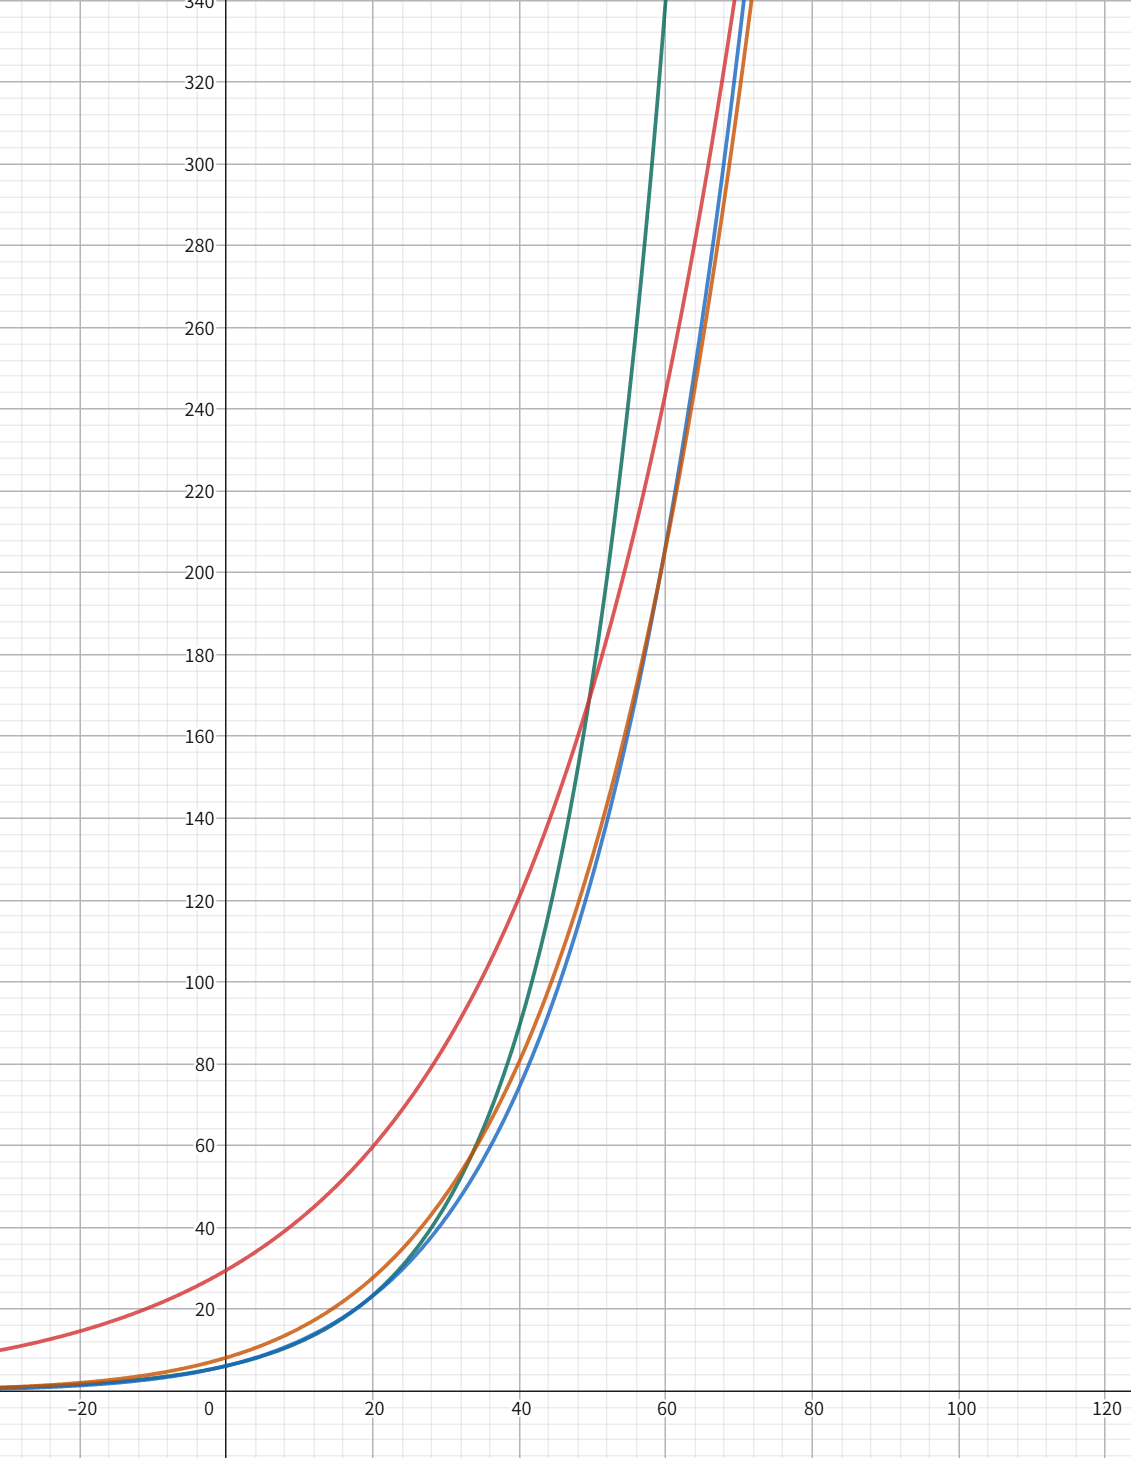
\includegraphics[width=0.8\textwidth]{image.png}
  \caption{Comparison of Saturated Vapor Pressure \( e_s(T) \) Calculated by Different Approximation Methods (Temperature Range: -20°C to 120°C)}
  \label{fig:es_comparison}
\end{figure}
Red Curve
  The function is  
  \[
  f_1(x) = 6.11 \times \exp(0.067 \times x)
  \]  
  where \( x \) is the temperature in degrees Celsius.
\\Blue Curve:
  The function is  
  \[
  f_2(x) = 6.11 \times \exp\!\left(\frac{2.46 \times 10^6}{461} \left(\frac{1}{273} - \frac{1}{x+273}\right)\right)
  \]  
  Here, the temperature \( x \) (in °C) is converted to Kelvin by using \( x+273 \).
\\Orange Curve:
  The function is  
  \[
  f_3(x) = 1000 \times \exp\!\left(\frac{2.26 \times 10^6}{461 \times 373^2}(x-100)\right)
  \]  
  This function is a linearized approximation around 100°C.
\\Green Curve:
  The function is  
  \[
  f_4(x) = 1000 \times \exp\!\left(\frac{2.26 \times 10^6}{461} \left(\frac{1}{373} - \frac{1}{x+273}\right)\right)
  \]  
  This function uses the Clausius-Clapeyron relation normalized at 100°C.

(3)

\begin{enumerate}[label=(\alph*)]
  \item \textbf{Dry Air:} \\
  For dry air, the density is given by the ideal gas law:
  \[
  \rho_d = \frac{P}{R_d T},
  \]
  where 
  \[
  P = 10^5\,\text{Pa}, \quad T = 20^\circ\text{C} = 293\,\text{K}, \quad R_d = 287.05\,\text{J\,kg}^{-1}\text{K}^{-1}.
  \]
  Therefore,
  \[
  \rho_d = \frac{10^5}{287.05 \times 293} \approx 1.189\,\text{kg/m}^3.
  \]

  \item \textbf{Moist Air:} \\
 For moist air with mixing ratio $r = 15\text{ g kg}^{-1} = 0.015\text{ kg kg}^{-1}$:
    
    The total pressure is shared between dry air and water vapor:
    \begin{equation*}
    P = P_d + e
    \end{equation*}
    
    where $e$ is the partial pressure of water vapor. Using the mixing ratio relation:
    \begin{equation*}
    r = \frac{M_v}{M_d} \frac{e}{P_d} = 0.622 \frac{e}{P_d}
    \end{equation*}
    
    Solving for $e$:
    \begin{equation*}
    e = \frac{r \cdot P_d}{0.622} = \frac{r(P - e)}{0.622}
    \end{equation*}
    \begin{equation*}
    e = \frac{rP}{0.622 + r} = \frac{0.015 \times 10^5}{0.622 + 0.015} \approx 2354.79\text{ Pa}
    \end{equation*}
    
    Therefore, $P_d = P - e = 10^5 - 2354.79 = 97645.21\text{ Pa}$
    
    The density of moist air is:
    \begin{equation*}
    \rho_{\text{moist}} = \frac{P_d}{R_d T} + \frac{e}{R_v T} \approx 1.178\text{ kg m}^{-3}
    \end{equation*}
    
  \end{enumerate}
  Thus, the moist air (approximately \(1.178\,\text{kg/m}^3\)) is slightly less dense than the dry air (approximately \(1.189\,\text{kg/m}^3\)) by \(0.011\text{kg/m}^3\) at the same temperature and pressure.
  \\(4)
  \begin{enumerate}[label=(\alph*)]
    \item At $T = 27°\text{C} = 300\text{ K}$ and $P = 10^5\text{ Pa}$:
    
    Using the Clausius-Clapeyron equation, the saturation vapor pressure is:
    \begin{equation*}
    e_s = 6.11 \exp\left(\frac{L}{R_v}\left(\frac{1}{273} - \frac{1}{T}\right)\right) \times 100\text{ Pa}
    \end{equation*}
    
    Approximating: $e_s \approx 3549\text{ Pa}$ at $27°\text{C}$.
    
    The saturation mixing ratio is:
    \begin{equation*}
    r_s = 0.622 \frac{e_s}{P - e_s} = 0.622 \times \frac{35749}{10^5 - 3549}  \approx 0.0229\text{ kg/kg}
    \end{equation*}
    
    \item At $T = -70°\text{C} = 203\text{ K}$ and $P = 2 \times 10^4\text{ Pa}$:
    \begin{equation*}
e_s(T) = e_0 \exp\left(\frac{L_s}{R_v}\left(\frac{1}{T_0} - \frac{1}{T}\right)\right)
\end{equation*} where $L_s = 2.83 \times 10^6\text{ J/kg}$
    \\$e_s \approx 0.26\text{ Pa}$ at $-70°\text{C}$.
    
    \begin{equation*}
    r_s = 0.622 \times \frac{0.26}{2 \times 10^4 - 0.26} \approx 0.622 \times \frac{0.26}{20000} \approx 8.1 \times 10^{-6}\text{ kg/kg}
    \end{equation*}
    
    \item The amount of water that condenses is:
    \begin{equation*}
    \Delta r = r_{\text{surface}} - r_{\text{top}} = 0.0229 - 8.1 \times 10^{-6} \approx 0.0229\text{ kg/kg}
    \end{equation*}
    
    \item Energy released per kg of air:
    \begin{equation*}
    E = \Delta r \times L = 0.0229 \times 2.3 \times 10^6 = 5.267 \times 10^4\text{ J/kg}
    \end{equation*}
    
    \item Mass of air needed to equal bomb energy:
    \begin{equation*}
    m = \frac{2.1 \times 10^{17}}{5.267 \times 10^4} = 3.987 \times 10^{12}\text{ kg}
    \end{equation*}
    
    \item For a cylinder of height $h = 500\text{ m}$ and density $\rho = 1.1\text{ kg/m}^3$:
    
    Volume needed:
    \begin{equation*}
    V = \frac{m}{\rho} = \frac{3.987 \times 10^{12}}{1.1} = 3.625\times 10^{12}\text{ m}^3
    \end{equation*}
    
    For a cylinder: $V = \pi r^2 h$, so:
    \begin{equation*}
    r = \sqrt{\frac{V}{\pi h}} = \sqrt{\frac{3.625\times 10^{12}}{\pi \times 500}} = \sqrt{2.308 \times 10^9} \approx 48041\text{ m} 
    \end{equation*}
    
    This cylinder has a radius of approximately 48 km, which is comparable to the size of a moderate tropical storm (typical storm radii range from 50-500 km). This demonstrates the enormous latent energy available in tropical oceanic air masses that powers these storms.
\end{enumerate}
\end{document}